\section{Empirical Test on EEG Measurements}
Consider now the same estimation of the number of active sources, $k$, but from the real EEG measurements. 
For this estimation one can not compare the estimation to the real sources as in the previous section.
Hence, the replica count method is just applied an estimation $\hat{\mathbf{X}}_{\text{main}}$ of real EEG measurements and a conclusion is made from the observed result.

The source signal estimation is performed on segment 10 from the \texttt{S1\_Cclean} EEG data set, where every second sensor is removed to achieve the case where $M < N$. 
Specifically $\hat{\mathbf{X}}_{\text{main}}$ is computed given $k = N$ and $\hat{\textbf{A}}_{\text{fix}}$ resulting from segment of EEG measurements specified by $M = 1/2 N = 13$. 

Figure \ref{fig:eeg_k} visualize the recovered source matrix $\hat{\mathbf{X}}_{\text{main}}$ from time segment $s = 10$ for $M = 13$ and $k = N = 27$. For visual simplicity only 8 out of 27 sources are visualized.
\begin{figure}[H]
    \centering
	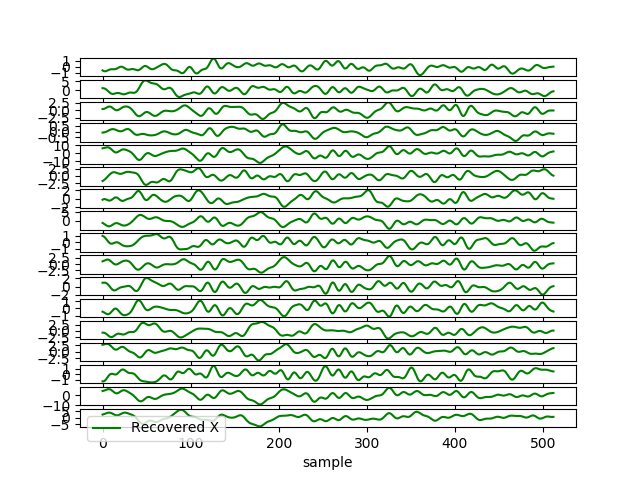
\includegraphics[scale=0.5]{figures/ch_estimate/eeg_k_timeseg_10.png}
	\caption{The recovered source matrix $\hat{\mathbf{X}}_{\text{main}}$ from time segment $s = 10$ from \texttt{S1\_Cclean} for $M = 13$ and $k = N = 27$. Note only the first 8 rows of $\hat{\mathbf{X}}_{\text{main}}$ is plotted for simplicity.}
	\label{fig:eeg_k}
\end{figure}
\noindent
From figure \ref{fig:eeg_k} it is seen that all $10$ source signals appears to be active -- the non visualized source signals do also appears to be active.
Furthermore, there seem not to be any visible indication of an active source being non-active, with respect to being a direct replica. 

By applying the replica count method to $\hat{\mathbf{X}}_{\text{main}}$  from figure \ref{fig:eeg_k} only one source signal is not considered replicas. 
This potentially active source signal is found in row 13, the last row plot on figure \ref{fig:eeg_k}. 
This leads to the conclusion that for time segment $s = 10$ with system specification $M = 13$ for the \texttt{S1\_Cclean} EEG data set only have $k = 1$ active sources. 



